\section{Informe Power BI} 
\begin{flushleft}


\begin{itemize}
\textbf{Ejercicio 1: Crear relaciones}\\
\textbf{ }\\
\textbf{Tarea 1:  } Relaciones automáticas\\
\textbf{ }\\

 1. Ingresar a Power BI Desktop.\\
 2. En la Ventana de Power BI Desktop, click en Obtener Datos (Get Data)\\
 3. En el cuadro de dialogo Obtener Datos (Get Data), asegurarse que Excel esta seleccionado y hacer click
en Conectar (Connect).\\
 4. En el cuadro de dialogo Abrir (Open), buscar el archivo Adventure Works Sales Data.xlsx, y luego hacer
click en Abrir (Open).\\
\textbf{ }\\
\begin{center}
	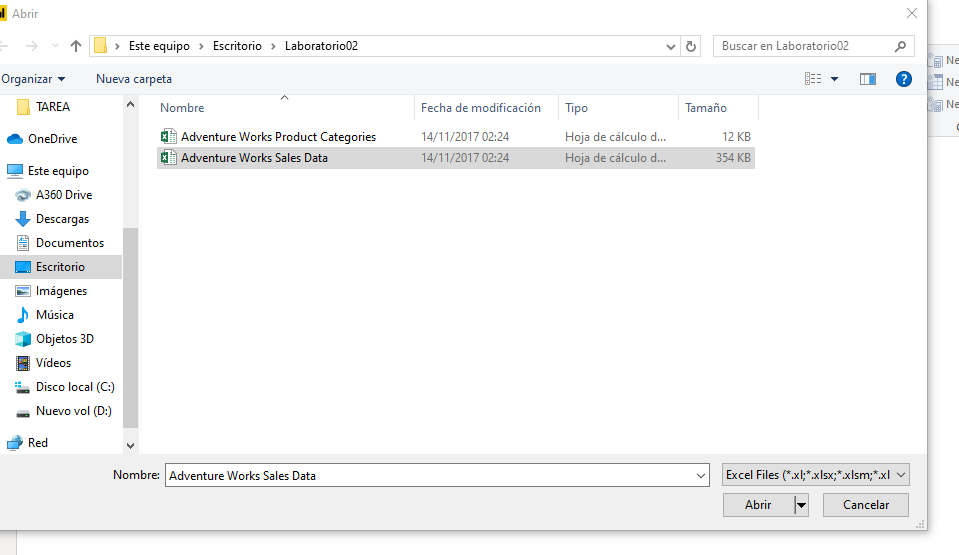
\includegraphics[width=20cm]{./Imagenes/img1} 
	\end{center}
\textbf{ }\\
\textbf{ }\\
\textbf{ }\\
\textbf{ }\\
\textbf{ }\\
\textbf{ }\\
\textbf{ }\\
\textbf{ }\\
\textbf{ }\\
\textbf{ }\\
\textbf{ }\\
\textbf{ }\\
5. En el cuadro de dialogo Explorador (Navigator), seleccionar las hojas DimCurrency, DimCustomer,
DimDate, DimProduct, DimPromotion, DimSalesTerritory, y FactInternetSales.\\
6. Hacer click en Cargar (Load).\\
\textbf{ }\\
\begin{center}
	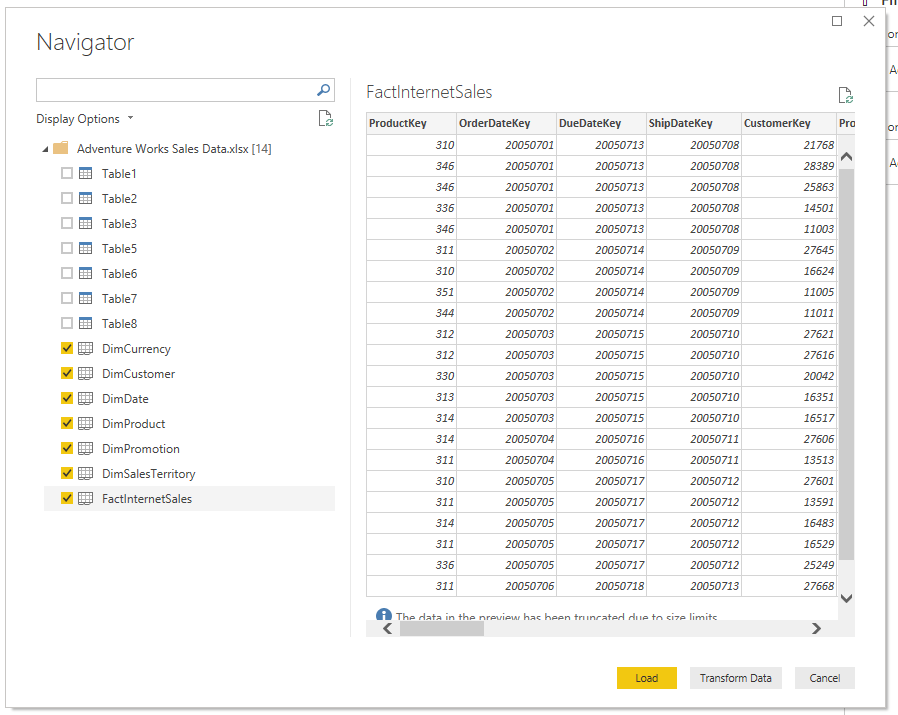
\includegraphics[width=20cm]{./Imagenes/img2} 
	\end{center}
\textbf{ }\\
\textbf{ }\\
\textbf{ }\\
\textbf{ }\\
\textbf{ }\\
\textbf{ }\\
\textbf{ }\\
\textbf{ }\\
\textbf{ }\\
\textbf{ }\\
7. En el panel de vistas a mano derecho, hacer click en Relaciones (Relationships).\\
8. En el menú principal, hacer click en Administrar relaciones (Manage Relationships).\\
9. En el cuadro de Administrar relaciones (Manage Relationships), hacer click en Nueva (New).\\
\textbf{ }\\
\begin{center}
	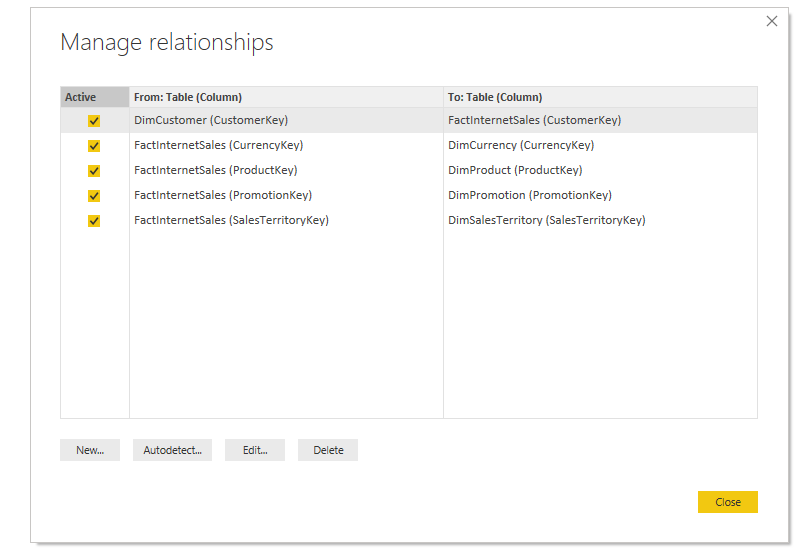
\includegraphics[width=20cm]{./Imagenes/img3} 
	\end{center}
\textbf{ }\\
\textbf{ }\\
\textbf{ }\\
\textbf{ }\\
\textbf{ }\\
\textbf{ }\\
\textbf{ }\\
\textbf{ }\\
\textbf{ }\\
\textbf{ }\\
\textbf{ }\\
\textbf{ }\\
\textbf{ }\\
\textbf{ }\\
\textbf{ }\\
10. En el cuadro de Administrar relaciones (Manage Relationships), en la lista de tablas superior, hacer click
en FactInternetSales. Cuando la vista previa de la table aparezca hacer click en la columna
OrderDateKey.\\
\textbf{ }\\
\begin{center}
	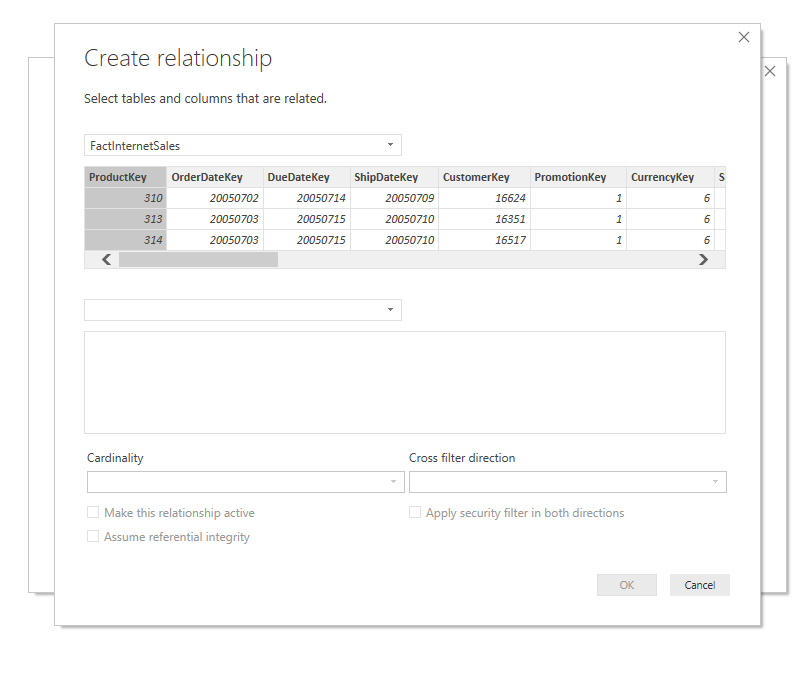
\includegraphics[width=20cm]{./Imagenes/img4} 
	\end{center}
\textbf{ }\\
\textbf{ }\\
\textbf{ }\\
\textbf{ }\\
\textbf{ }\\
\textbf{ }\\
\textbf{ }\\
\textbf{ }\\
\textbf{ }\\
\textbf{ }\\
\textbf{ }\\
11. En la lista de table inferior, hacer click en DimDate. Cuando la vista previa de la table aparezca hacer click
en la columna DateKey.\\
12. Revisar que la cardinalidad (Cardinality) esta seleccionada para Muchos a Uno (Many to One (*:1)), que la
Dirección del filtro cruzado (Cross filter direction) es Sencilla (Single), y que la opción Hacer esta relación
activa (Make this relationship active) se encuentra seleccionada, luego hacer click en Aceptar (OK).\\
\textbf{ }\\
\begin{center}
	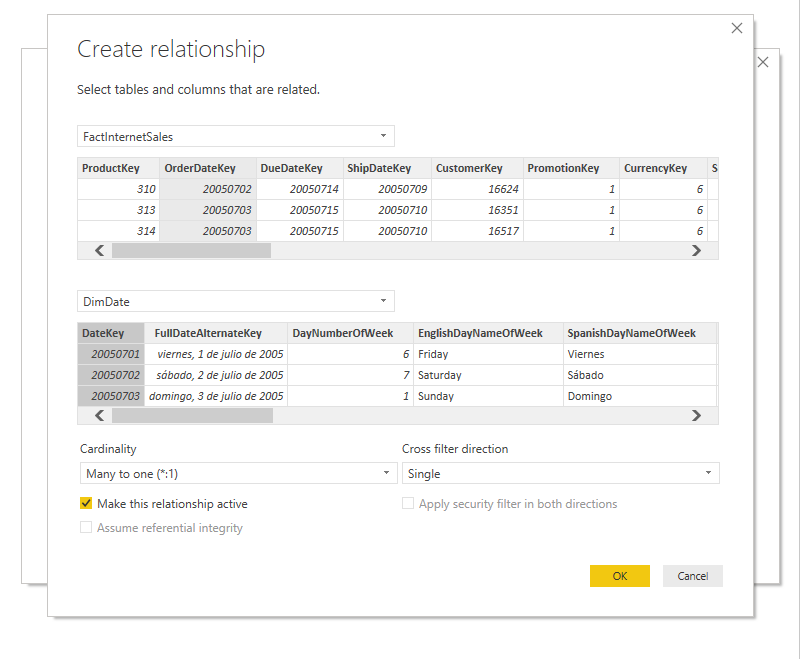
\includegraphics[width=20cm]{./Imagenes/img5} 
	\end{center}
\textbf{ }\\
\textbf{ }\\
\textbf{ }\\
\textbf{ }\\

13. En el cuadro de Administrar relaciones (Manage Relationships), hacer click en Cerrar (Close).\\
\textbf{ }\\

14. En el diagrama, en la tabla FactInternetSales, hacer click en la columna DueDateKey. Arrastrar la columna
DueDateKey a la columna DateKey de la tabla DimDate.\\
15. En el diagrama, en la tabla FactInternetSales, hacer click en la columna ShipDateKey. Arrastrar la
columna ShipDateKey a la columna DateKey de la tabla DimDate.\\
\textbf{ }\\
\begin{center}
	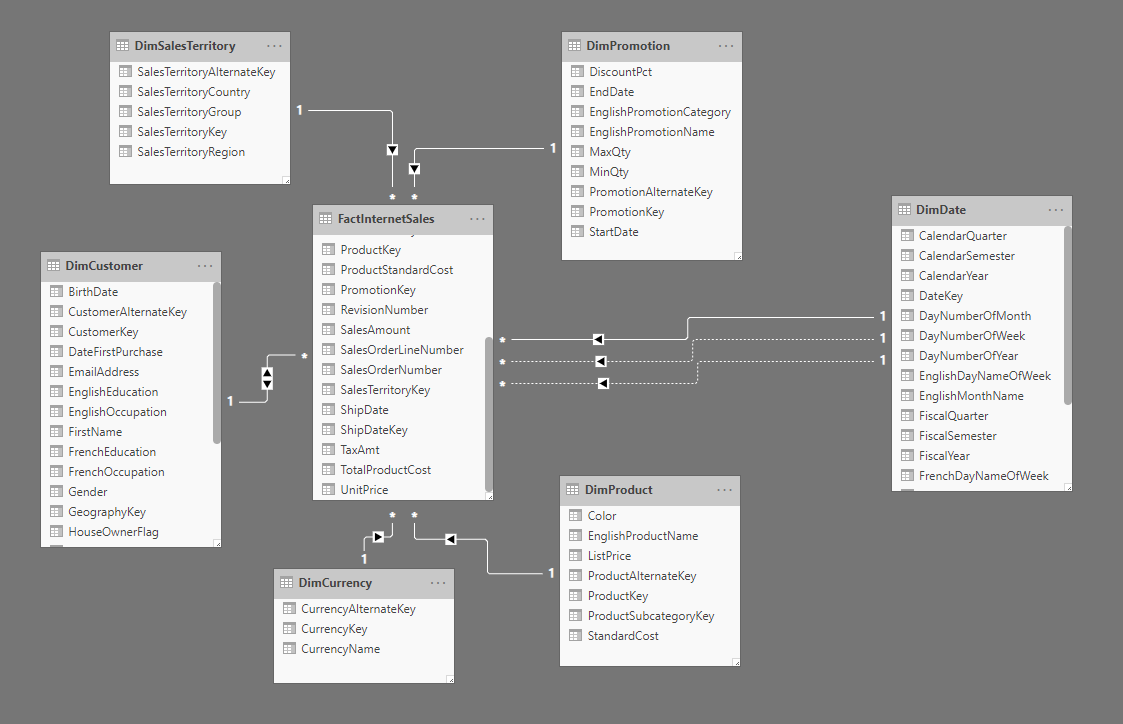
\includegraphics[width=20cm]{./Imagenes/img6} 
	\end{center}
\textbf{ }\\

16. En el menú principal, hacer click en Administrar relaciones (Manage Relationships)\\

17. En el cuadro de Administrar relaciones (Manage Relationships), hacer doble click en la relación
FactInternetSales (CurrencyKey).\\
18. En la lista de Dirección de Filtro Cruzado (Cross filter direction), hacer click en Sencilla (Single), luego
hacer click en Aceptar (OK).\\
19. En el cuadro de Administrar relaciones (Manage Relationships), hacer doble click en la relación
FactInternetSales (ProductKey).\\
20. En la lista de Dirección de Filtro Cruzado (Cross filter direction), hacer click en Sencilla (Single), luego
hacer click en Aceptar (OK).\\
21. En el cuadro de Administrar relaciones (Manage Relationships), hacer doble click en la relación
FactInternetSales (PromotionKey).\\
22. En la lista de Dirección de Filtro Cruzado (Cross filter direction), hacer click en Sencilla (Single), luego
hacer click en Aceptar (OK).\\
23. En el cuadro de Administrar relaciones (Manage Relationships), hacer doble click en la relación
FactInternetSales (SalesTerritoryKey).\\
24. En la lista de Dirección de Filtro Cruzado (Cross filter direction), hacer click en Sencilla (Single), luego
hacer click en Aceptar (OK).\\
25. En el cuadro de Administrar relaciones (Manage Relationships), hacer click en Cerrar (Close)..\\
(Delete)..\\

\textbf{ }\\
\begin{center}
	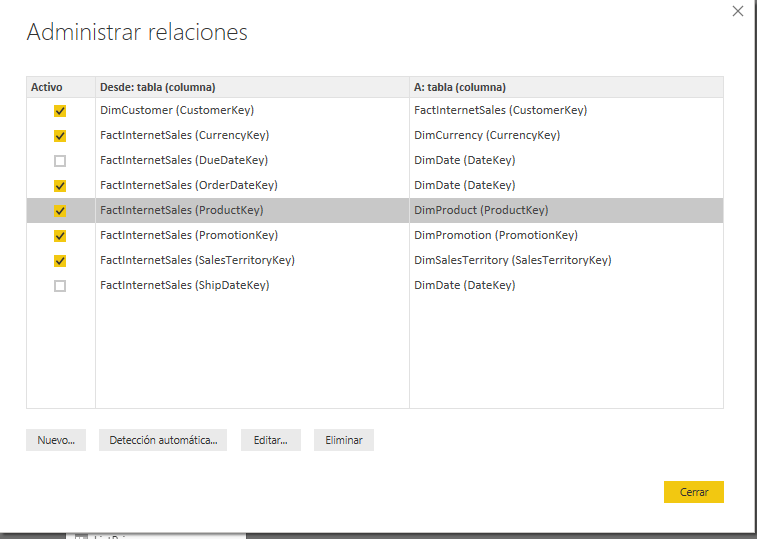
\includegraphics[width=20cm]{./Imagenes/img7} 
	\end{center}
\textbf{ }\\
\textbf{ }\\
\textbf{ }\\
\textbf{ }\\
\textbf{ }\\
\textbf{ }\\
\textbf{ }\\
\textbf{ }\\
\textbf{ }\\
\textbf{ }\\
\textbf{ }\\
\textbf{ }\\
\textbf{ }\\
\textbf{ }\\

\textbf{ }\\

26. Hacer click en la línea de relación entre FactInternetSales and DimCustomer y presionar Borrar (Delete).\\
27. En el cuadro de dialogo Eliminar relación (Delete Relationship), hacer click en Borrar (Delete)..\\
\textbf{ }\\

\begin{center}
	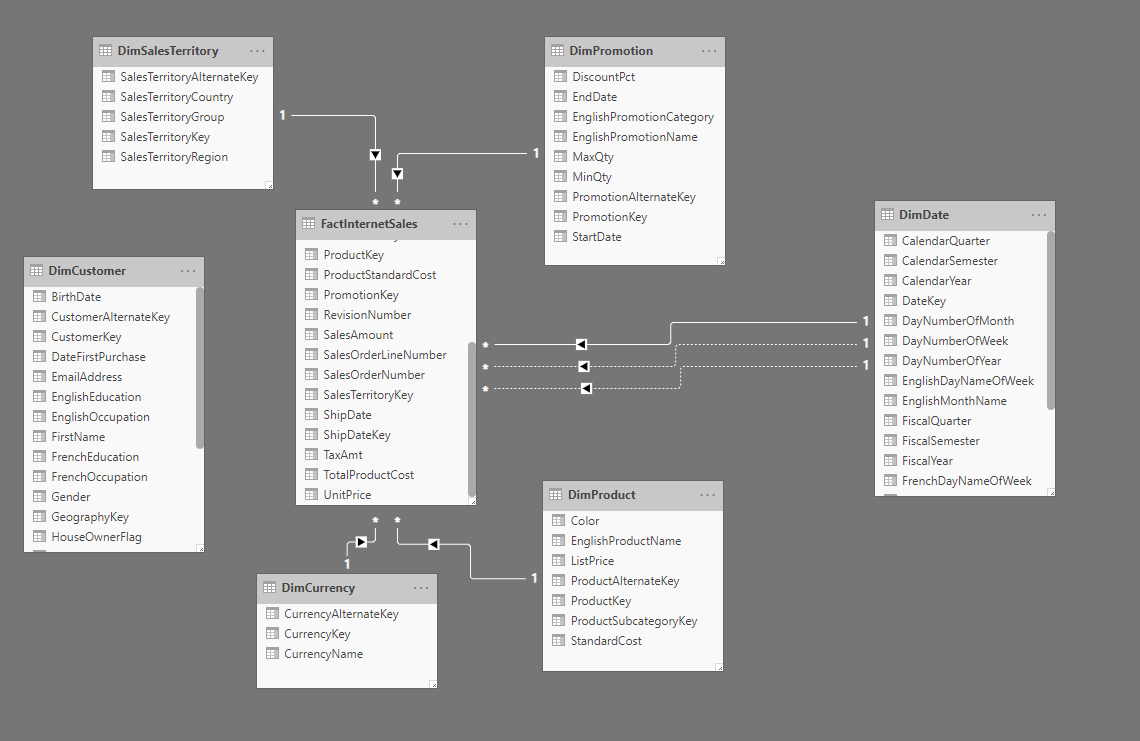
\includegraphics[width=20cm]{./Imagenes/img8} 
	\end{center}
\textbf{ }\\
\textbf{ }\\
\textbf{ }\\
\textbf{ }\\
\textbf{ }\\
\textbf{ }\\
\textbf{ }\\
\textbf{ }\\
\textbf{ }\\
\textbf{ }\\
\textbf{ }\\
\textbf{ }\\
\textbf{ }\\
\textbf{ }\\
28. En el menú principal, hacer click en Administrar relaciones (Manage Relationships).\\
29. En el cuadro de Administrar relaciones (Manage Relationships), hacer click en Nueva (New).\\
30. En la lista de tablas superior, hacer click en FactInternetSales. Luego hacer click en la columna
CustomerKey en la vista de datos previa.\\
31. En la lista de tablas superior, hacer click en DimCustomer, y hacer click CustomerKey en la vista de datos
previa.\\
32. En la lista de Cardinalidad (Cardinality), hacer click en Muchos a Uno (Many to One (*:1)), y luego hacer
click en Aceptar (OK).\\
\textbf{ }\\

\begin{center}
	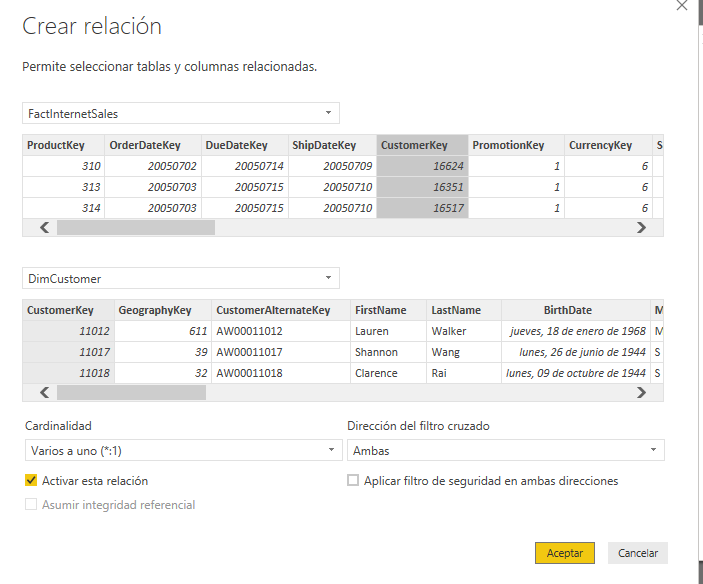
\includegraphics[width=20cm]{./Imagenes/img9} 
	\end{center}
\textbf{ }\\

\textbf{ }\\
\textbf{ }\\
\textbf{ }\\
33. En el cuadro de Administrar relaciones (Manage Relationships), hacer click en Cerrar (Close).\\
\textbf{ }\\

\begin{center}
	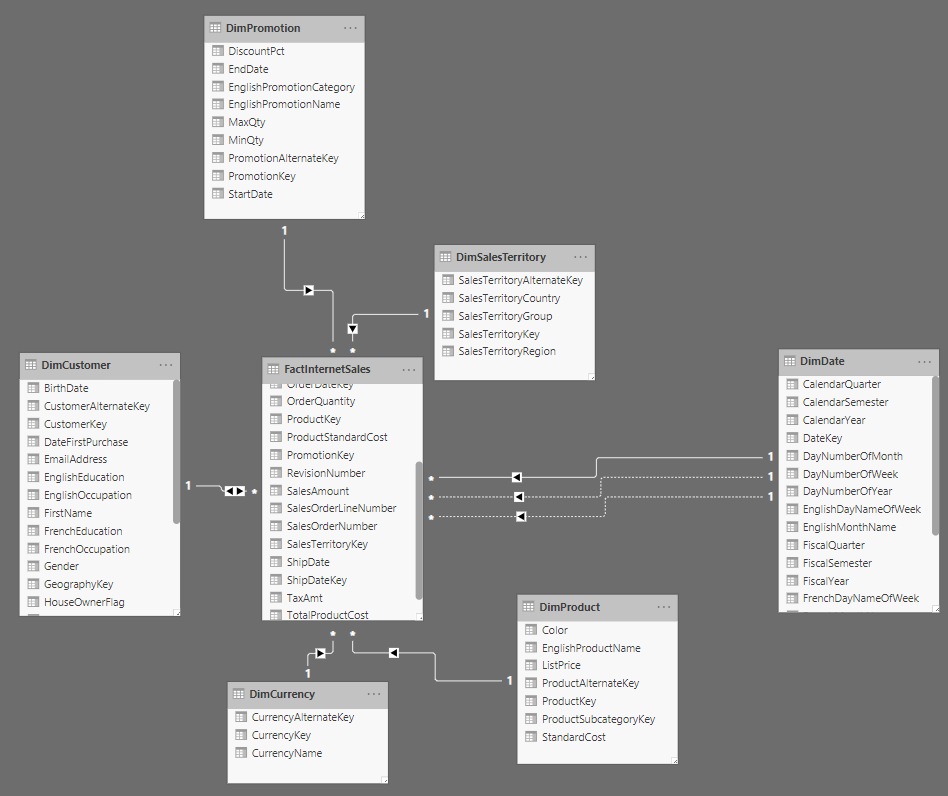
\includegraphics[width=20cm]{./Imagenes/img10} 
	\end{center}
\textbf{ }\\

34. Hacer click en Guardar (Save), y cuargar el archive como Ventas Adventure Works.pbix.\\


\textbf{ }\\
\textbf{ }\\
\textbf{ }\\
\textbf{ }\\
\textbf{ }\\
\textbf{ }\\
\textbf{ }\\
\textbf{ }\\
\textbf{ }\\
\textbf{Tarea 2:  } Relaciones manuales
\textbf{ }\\
\textbf{ }\\
1. En la Ventana de Power BI Desktop, click en Obtener Datos (Get Data) y luego en Excel.\\
2. Abrir el archivo Adventure Works Product Categories.xlsx\\
\textbf{ }\\
\begin{center}
	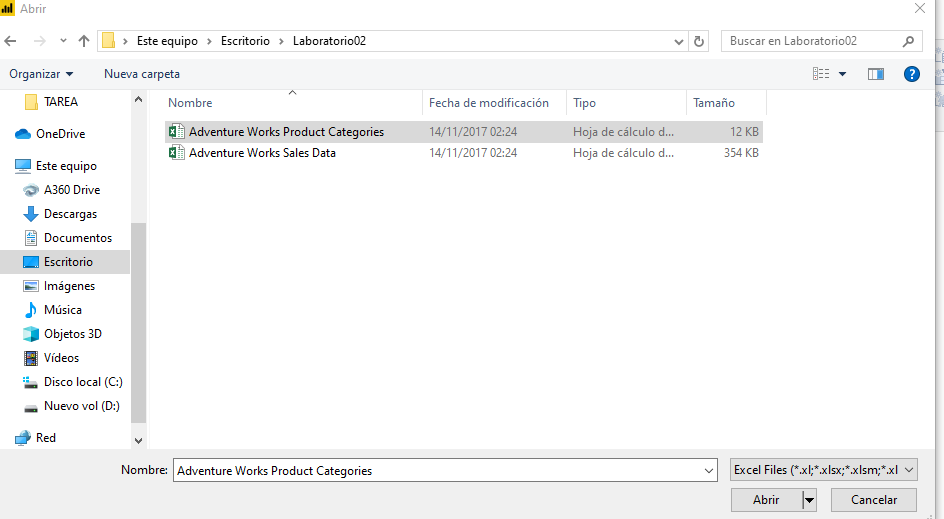
\includegraphics[width=20cm]{./Imagenes/img20} 
	\end{center}
\textbf{ }\\

\textbf{ }\\
\textbf{ }\\
\textbf{ }\\
\textbf{ }\\
\textbf{ }\\
\textbf{ }\\
\textbf{ }\\
\textbf{ }\\
\textbf{ }\\
\textbf{ }\\
\textbf{ }\\
\textbf{ }\\
\textbf{ }\\
\textbf{ }\\
\textbf{ }\\
\textbf{ }\\
\textbf{ }\\
\textbf{ }\\
\textbf{ }\\
3. En el cuadro de dialogo Explorador (Navigator), seleccionar las hojas DimProductCategory, and
DimProductSubcategory, y luego hacer click en Cargar (Load).
\textbf{ }\\
\begin{center}
	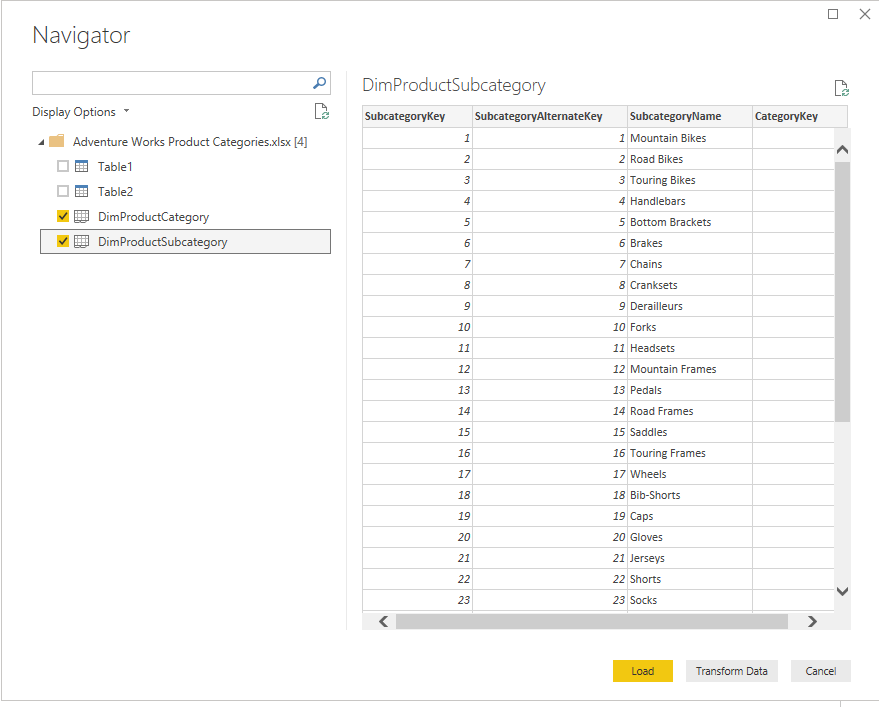
\includegraphics[width=20cm]{./Imagenes/img21} 
	\end{center}
\textbf{ }\\
\textbf{ }\\
\textbf{ }\\
\textbf{ }\\
\textbf{ }\\
\textbf{ }\\
\textbf{ }\\
\textbf{ }\\
\textbf{ }\\
\textbf{ }\\
\textbf{ }\\
\textbf{ }\\
\textbf{ }\\
4. En el panel de Relaciones, revisar la relación que Power BI ha creado entre las dos tablas.\\
\textbf{ }\\
\begin{center}
	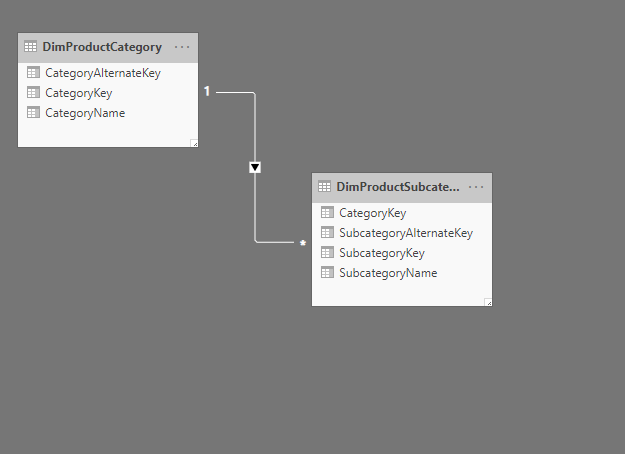
\includegraphics[width=20cm]{./Imagenes/img22} 
	\end{center}
\textbf{ }\\
\textbf{ }\\
\textbf{ }\\
\textbf{ }\\
\textbf{ }\\
\textbf{ }\\
\textbf{ }\\
\textbf{ }\\
\textbf{ }\\
\textbf{ }\\
\textbf{ }\\
\textbf{ }\\
\textbf{ }\\
\textbf{ }\\
\textbf{ }\\
\textbf{ }\\
5. Hacer click en la línea de la relación entre DimProductCategory, y DimProductSubcategory, y seleccionar. \\

6. En el cuadro de dialogo Eliminar relación (Delete Relationship), hacer click en Borrar (Delete).\\
\textbf{ }\\
\begin{center}
	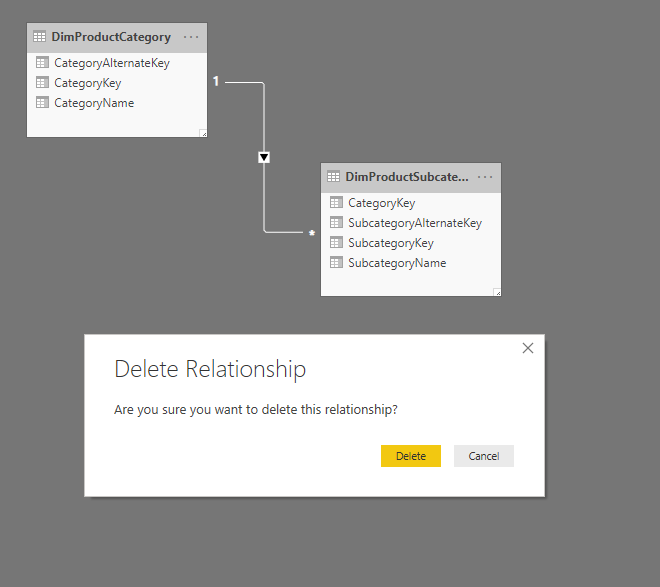
\includegraphics[width=20cm]{./Imagenes/img23} 
	\end{center}
\textbf{ }\\

\textbf{ }\\
\begin{center}
	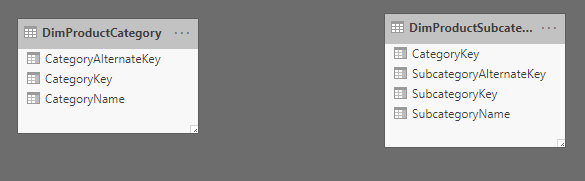
\includegraphics[width=20cm]{./Imagenes/img24} 
	\end{center}
\textbf{ }\\

7. Arrastrar la columna CategoryKey en la tabla DimProductSubcategory a la columna Category en la tabla
DimProductCategory, para crear una relación Muchos a uno (Many to One (*:1)), y una dirección de filtro
cruzado (Cross filter
direction) en ambos.\\
\textbf{ }\\
\begin{center}
	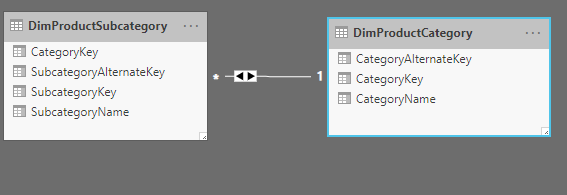
\includegraphics[width=20cm]{./Imagenes/img25} 
	\end{center}
\textbf{ }\\

\textbf{ }\\
\textbf{ }\\
\textbf{ }\\
\textbf{ }\\
\textbf{ }\\
\textbf{ }\\
\textbf{ }\\
\textbf{ }\\
\textbf{ }\\
\textbf{ }\\
\textbf{ }\\
\textbf{ }\\
\textbf{ }\\
\textbf{ }\\
\textbf{ }\\
8. En la tabla DimProduct, arrastrar la columna ProductSubcategoryKey a la columna SubcategoryKey en la
tabla DimProductSubcategory, para crear una relación de Muchos a Uno (Many to One (*:1)), y una
dirección de filtro cruzado (Cross filter direction) en ambos.\\
\textbf{ }\\
\begin{center}
	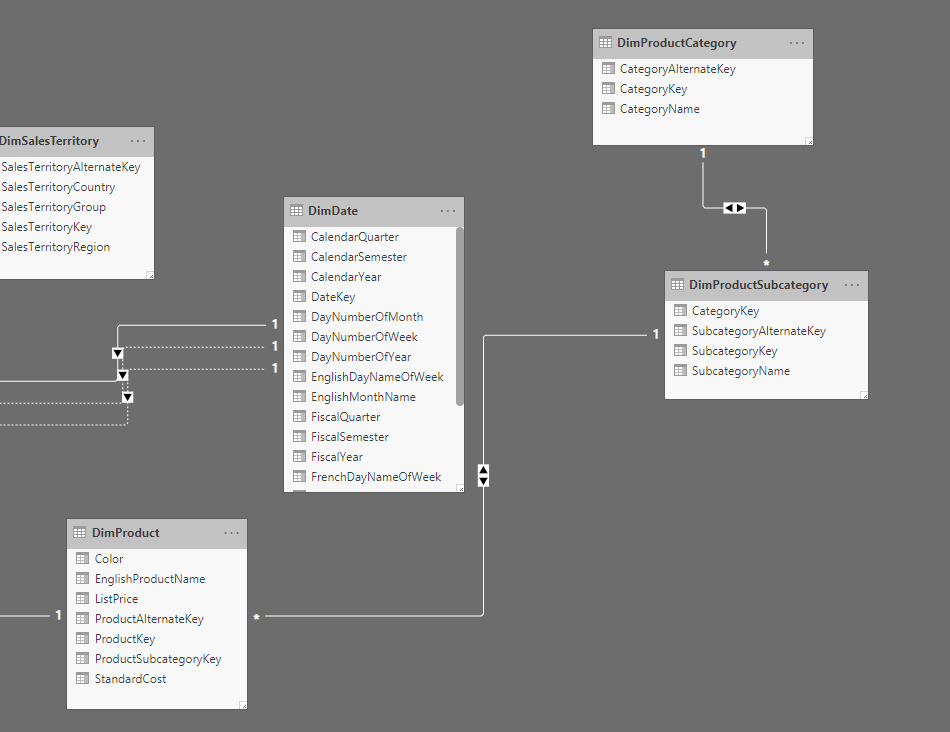
\includegraphics[width=20cm]{./Imagenes/img26} 
	\end{center}
\textbf{ }\\
9. Hacer click en Guardar\\
\textbf{ }\\
\textbf{ }\\
\textbf{ }\\
\textbf{ }\\
\textbf{ }\\
\textbf{ }\\
\textbf{ }\\
\textbf{ }\\
\textbf{ }\\
\textbf{ }\\
\textbf{Ejercicio 2: Cálculos}\\
\textbf{ }\\
\textbf{Tarea 1:  } Agregar una columna calculada
\textbf{ }\\
1. En Power BI Desktop, haga clic en Datos en el panel de vistas en el lado izquierdo.\\
2. En el panel Campos, haga clic en DimCustomer.\\
\textbf{ }\\
\begin{center}
	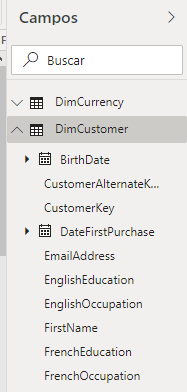
\includegraphics[width=4cm]{./Imagenes/img30} 
	\end{center}
\textbf{ }\\
3. En la cinta de Modelado, en el grupo Cálculos, haga clic en Nueva columna.\\
\textbf{ }\\
\begin{center}
	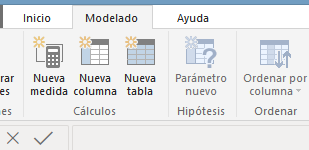
\includegraphics[width=6cm]{./Imagenes/img31} 
	\end{center}
\textbf{ }\\
4. En la barra de fórmulas, resalte Columna = y escriba: 
IncomeStatus = IF (DimCustomer[YearlyIncome] < 25000, "Lower Income",
IF (AND(DimCustomer[YearlyIncome] >= 25000, DimCustomer[YearlyIncome] < 60000),
"Middle Income",
IF (AND(DimCustomer[YearlyIncome] >= 60000, DimCustomer[YearlyIncome] < 100000),
"Higher Income",
IF (DimCustomer[YearlyIncome] >= 100000, "Very High Income", "Other"))))\\
5. Presione Entrar.\\
\textbf{ }\\
\begin{center}
	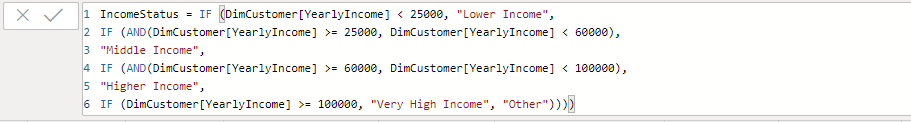
\includegraphics[width=17cm]{./Imagenes/img32} 
	\end{center}
\textbf{ }\\
\textbf{ }\\
6. En la cinta de Modelado, en el grupo Cálculos, haga clic en Nueva columna.\\
7. En la barra de fórmulas, resalte Columna = y escriba:
DaysSinceFirstPurchase = DATEDIFF(DimCustomer[DateFirstPurchase], TODAY(), DAY)\\
8. Presione Entrar.\\
\textbf{ }\\
\begin{center}
	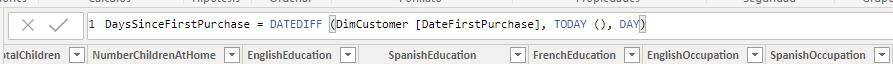
\includegraphics[width=17cm]{./Imagenes/img33} 
	\end{center}
\textbf{ }\\



9. En la cinta de Modelado, en el grupo Cálculos, haga clic en Nueva columna.\\
10. En la barra de fórmulas, resalte Columna = y escriba:
FullName = [FirstName] \& " " \& [LastName]\\
11. Presione Entrar.\\
\textbf{ }\\
\begin{center}
	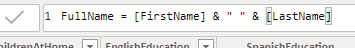
\includegraphics[width=13cm]{./Imagenes/img34} 
	\end{center}
\textbf{ }\\


12. En la cinta de Modelado, en el grupo Cálculos, haga clic en Nueva columna.\\
13. En la barra de fórmulas, resalte Columna = y escriba:
MaleFemale = IF([Gender] = "M", "Male", "Female")\\
14. Presione Entrar.\\
\textbf{ }\\
\begin{center}
	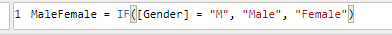
\includegraphics[width=13cm]{./Imagenes/img35} 
	\end{center}
\textbf{ }\\




15. En la cinta de Modelado, en el grupo Cálculos, haga clic en Nueva columna.\\
16. En la barra de fórmulas, resalte Columna = y escriba:
Relationship = IF([MaritalStatus] = "M", "Married", "Single")\\
17. Presione Entrar.\\
\textbf{ }\\
\begin{center}
	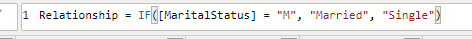
\includegraphics[width=13cm]{./Imagenes/img36} 
	\end{center}
\textbf{ }\\
\textbf{ }\\
\textbf{ }\\
\textbf{ }\\
\textbf{ }\\
\textbf{ }\\
\textbf{ }\\
\textbf{ }\\
\textbf{ }\\
\textbf{ }\\
\textbf{ }\\
\textbf{ }\\
\textbf{ }\\

18. En el panel Campos, haga clic en DimProductSubcategory.\\
\textbf{ }\\
\begin{center}
	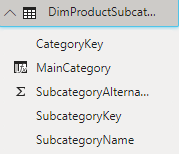
\includegraphics[width=5cm]{./Imagenes/img38} 
	\end{center}
\textbf{ }\\

19. En la cinta de Modelado, en el grupo Cálculos, haga clic en Nueva columna.\\
\textbf{ }\\
\begin{center}
	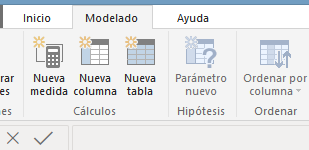
\includegraphics[width=13cm]{./Imagenes/img37} 
	\end{center}
\textbf{ }\\

20. En la barra de fórmulas, resalte Columna = y escriba:
MainCategory = RELATED (DimProductCategory [CategoryName])\\
21. Presione Entrar.\\
\textbf{ }\\
\begin{center}
	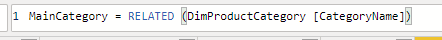
\includegraphics[width=13cm]{./Imagenes/img39} 
	\end{center}
\textbf{ }\\

22. En el panel Campos, haga clic en DimPromotion.\\
23. En la cinta de Modelado, en el grupo Cálculos, haga clic en Nueva columna.\\
24. En la barra de fórmulas, resalte Columna = y escriba:
PromotionLengthDays = DATEDIFF (DimPromotion [StartDate], DimPromotion [EndDate], DAY)\\
25. Presione Entrar.\\
\textbf{ }\\
\begin{center}
	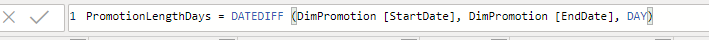
\includegraphics[width=13cm]{./Imagenes/img40} 
	\end{center}
\textbf{ }\\
\textbf{ }\\
\textbf{ }\\
\textbf{ }\\
\textbf{ }\\

26. En el panel Campos, haga clic en FactInternetSales.\\
27. En la cinta de Modelado, en el grupo Cálculos, haga clic en Nueva columna.\\
28. En la barra de fórmulas, resalte Columna = y escriba:
Beneficio = MONEDA (FactInternetSales [UnitPrice] -
FactInternetSales [ProductStandardCost])\\
29. Pressionar Enter.\\
\textbf{ }\\
\begin{center}
	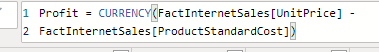
\includegraphics[width=13cm]{./Imagenes/img41} 
	\end{center}
\textbf{ }\\
30. Cerrar Power BI Desktop, salvando cualquier cambio.
\end{itemize} 


\end{flushleft}